%==============================================================================
% tento soubor pouzijte jako zaklad
% this file should be used as a base for the thesis
% Autoři / Authors: 2008 Michal Bidlo, 2019 Jaroslav Dytrych
% Kontakt pro dotazy a připomínky: sablona@fit.vutbr.cz
% Contact for questions and comments: sablona@fit.vutbr.cz
%==============================================================================
% kodovani: UTF-8 (zmena prikazem iconv, recode nebo cstocs)
% encoding: UTF-8 (you can change it by command iconv, recode or cstocs)
%------------------------------------------------------------------------------
% zpracování / processing: make, make pdf, make clean
%==============================================================================
% Soubory, které je nutné upravit nebo smazat: / Files which have to be edited or deleted:
%   projekt-20-literatura-bibliography.bib - literatura / bibliography
%   projekt-01-kapitoly-chapters.tex - obsah práce / the thesis content
%   projekt-01-kapitoly-chapters-en.tex - obsah práce v angličtině / the thesis content in English
%   projekt-30-prilohy-appendices.tex - přílohy / appendices
%   projekt-30-prilohy-appendices-en.tex - přílohy v angličtině / appendices in English
%==============================================================================
\documentclass[slovak]{fitthesis} % bez zadání - pro začátek práce, aby nebyl problém s překladem
%\documentclass[english]{fitthesis} % without assignment - for the work start to avoid compilation problem
%\documentclass[zadani]{fitthesis} % odevzdani do wisu a/nebo tisk s barevnými odkazy - odkazy jsou barevné
%\documentclass[english,zadani]{fitthesis} % for submission to the IS FIT and/or print with color links - links are color
%\documentclass[zadani,print]{fitthesis} % pro černobílý tisk - odkazy jsou černé
%\documentclass[english,zadani,print]{fitthesis} % for the black and white print - links are black
%\documentclass[zadani,cprint]{fitthesis} % pro barevný tisk - odkazy jsou černé, znak VUT barevný
%\documentclass[english,zadani,cprint]{fitthesis} % for the print - links are black, logo is color
% * Je-li práce psaná v anglickém jazyce, je zapotřebí u třídy použít 
%   parametr english následovně:
%   If thesis is written in English, it is necessary to use 
%   parameter english as follows:
%      \documentclass[english]{fitthesis}
% * Je-li práce psaná ve slovenském jazyce, je zapotřebí u třídy použít 
%   parametr slovak následovně:
%   If the work is written in the Slovak language, it is necessary 
%   to use parameter slovak as follows:
%      \documentclass[slovak]{fitthesis}
% * Je-li práce psaná v anglickém jazyce se slovenským abstraktem apod., 
%   je zapotřebí u třídy použít parametry english a enslovak následovně:
%   If the work is written in English with the Slovak abstract, etc., 
%   it is necessary to use parameters english and enslovak as follows:
%      \documentclass[english,enslovak]{fitthesis}

% Základní balíčky jsou dole v souboru šablony fitthesis.cls
% Basic packages are at the bottom of template file fitthesis.cls
% zde můžeme vložit vlastní balíčky / you can place own packages here

% Kompilace po částech (rychlejší, ale v náhledu nemusí být vše aktuální)
% Compilation piecewise (faster, but not all parts in preview will be up-to-date)
% \usepackage{subfiles}

% Nastavení cesty k obrázkům
% Setting of a path to the pictures
%\graphicspath{{obrazky-figures/}{./obrazky-figures/}}
%\graphicspath{{obrazky-figures/}{../obrazky-figures/}}

%---rm---------------
\renewcommand{\rmdefault}{lmr}%zavede Latin Modern Roman jako rm / set Latin Modern Roman as rm
%---sf---------------
\renewcommand{\sfdefault}{qhv}%zavede TeX Gyre Heros jako sf
%---tt------------
\renewcommand{\ttdefault}{lmtt}% zavede Latin Modern tt jako tt

% vypne funkci šablony, která automaticky nahrazuje uvozovky,
% aby nebyly prováděny nevhodné náhrady v popisech API apod.
% disables function of the template which replaces quotation marks
% to avoid unnecessary replacements in the API descriptions etc.
\csdoublequotesoff



\usepackage{url}


% =======================================================================
% balíček "hyperref" vytváří klikací odkazy v pdf, pokud tedy použijeme pdflatex
% problém je, že balíček hyperref musí být uveden jako poslední, takže nemůže
% být v šabloně
% "hyperref" package create clickable links in pdf if you are using pdflatex.
% Problem is that this package have to be introduced as the last one so it 
% can not be placed in the template file.
\ifWis
\ifx\pdfoutput\undefined % nejedeme pod pdflatexem / we are not using pdflatex
\else
  \usepackage{color}
  \usepackage[unicode,colorlinks,hyperindex,plainpages=false,pdftex]{hyperref}
  \definecolor{hrcolor-ref}{RGB}{223,52,30}
  \definecolor{hrcolor-cite}{HTML}{2F8F00}
  \definecolor{hrcolor-urls}{HTML}{092EAB}
  \hypersetup{
	linkcolor=hrcolor-ref,
	citecolor=hrcolor-cite,
	filecolor=magenta,
	urlcolor=hrcolor-urls
  }
  \def\pdfBorderAttrs{/Border [0 0 0] }  % bez okrajů kolem odkazů / without margins around links
  \pdfcompresslevel=9
\fi
\else % pro tisk budou odkazy, na které se dá klikat, černé / for the print clickable links will be black
\ifx\pdfoutput\undefined % nejedeme pod pdflatexem / we are not using pdflatex
\else
  \usepackage{color}
  \usepackage[unicode,colorlinks,hyperindex,plainpages=false,pdftex,urlcolor=black,linkcolor=black,citecolor=black]{hyperref}
  \definecolor{links}{rgb}{0,0,0}
  \definecolor{anchors}{rgb}{0,0,0}
  \def\AnchorColor{anchors}
  \def\LinkColor{links}
  \def\pdfBorderAttrs{/Border [0 0 0] } % bez okrajů kolem odkazů / without margins around links
  \pdfcompresslevel=9
\fi
\fi
% Řešení problému, kdy klikací odkazy na obrázky vedou za obrázek
% This solves the problems with links which leads after the picture
\usepackage[all]{hypcap}

% Informace o práci/projektu / Information about the thesis
%---------------------------------------------------------------------------
\projectinfo{
  %Prace / Thesis
  project={SP},            %typ práce BP/SP/DP/DR  / thesis type (SP = term project)
  year={2021},             % rok odevzdání / year of submission
  date=\today,             % datum odevzdání / submission date
  %Nazev prace / thesis title
  title.cs={Replikácia častí Platypus publikácie},  % název práce v češtině či slovenštině (dle zadání) / thesis title in czech language (according to assignment)
  title.en={Replication of parts of the Platypus publication}, % název práce v angličtině / thesis title in english
  %title.length={14.5cm}, % nastavení délky bloku s titulkem pro úpravu zalomení řádku (lze definovat zde nebo níže) / setting the length of a block with a thesis title for adjusting a line break (can be defined here or below)
  %sectitle.length={14.5cm}, % nastavení délky bloku s druhým titulkem pro úpravu zalomení řádku (lze definovat zde nebo níže) / setting the length of a block with a second thesis title for adjusting a line break (can be defined here or below)
  %dectitle.length={14.5cm}, % nastavení délky bloku s titulkem nad prohlášením pro úpravu zalomení řádku (lze definovat zde nebo níže) / setting the length of a block with a thesis title above declaration for adjusting a line break (can be defined here or below)
  %Autor / Author
  author.name={Patrik},   % jméno autora / author name
  author.surname={Németh},   % příjmení autora / author surname 
  %author.title.p={Bc.}, % titul před jménem (nepovinné) / title before the name (optional)
  %author.title.a={Ph.D.}, % titul za jménem (nepovinné) / title after the name (optional)
  %Ustav / Department
  department={UITS}, % doplňte příslušnou zkratku dle ústavu na zadání: UPSY/UIFS/UITS/UPGM / fill in appropriate abbreviation of the department according to assignment: UPSY/UIFS/UITS/UPGM
  % Školitel / supervisor
  supervisor.name={Kamil},   % jméno školitele / supervisor name 
  supervisor.surname={Malinka},   % příjmení školitele / supervisor surname
  supervisor.title.p={Mgr.},   %titul před jménem (nepovinné) / title before the name (optional)
  supervisor.title.a={Ph.D.},    %titul za jménem (nepovinné) / title after the name (optional)
  % Klíčová slova / keywords
  keywords.cs={Sem budou zapsána jednotlivá klíčová slova v českém (slovenském) jazyce, oddělená čárkami.}, % klíčová slova v českém či slovenském jazyce / keywords in czech or slovak language
  keywords.en={Sem budou zapsána jednotlivá klíčová slova v anglickém jazyce, oddělená čárkami.}, % klíčová slova v anglickém jazyce / keywords in english
  %keywords.en={Here, individual keywords separated by commas will be written in English.},
  % Abstrakt / Abstract
  abstract.cs={Do tohoto odstavce bude zapsán výtah (abstrakt) práce v českém (slovenském) jazyce.}, % abstrakt v českém či slovenském jazyce / abstract in czech or slovak language
  abstract.en={Do tohoto odstavce bude zapsán výtah (abstrakt) práce v anglickém jazyce.}, % abstrakt v anglickém jazyce / abstract in english
  %abstract.en={An abstract of the work in English will be written in this paragraph.},
  % Prohlášení (u anglicky psané práce anglicky, u slovensky psané práce slovensky) / Declaration (for thesis in english should be in english)
  declaration={Prohlašuji, že jsem tuto bakalářskou práci vypracoval samostatně pod vedením pana X...
Další informace mi poskytli...
Uvedl jsem všechny literární prameny, publikace a další zdroje, ze kterých jsem čerpal.},
  %declaration={I hereby declare that this Bachelor's thesis was prepared as an original work by the author under the supervision of Mr. X
% The supplementary information was provided by Mr. Y
% I have listed all the literary sources, publications and other sources, which were used during the preparation of this thesis.},
  % Poděkování (nepovinné, nejlépe v jazyce práce) / Acknowledgement (optional, ideally in the language of the thesis)
  acknowledgment={V této sekci je možno uvést poděkování vedoucímu práce a těm, kteří poskytli odbornou pomoc
(externí zadavatel, konzultant apod.).},
  %acknowledgment={Here it is possible to express thanks to the supervisor and to the people which provided professional help
%(external submitter, consultant, etc.).},
  % Rozšířený abstrakt (cca 3 normostrany) - lze definovat zde nebo níže / Extended abstract (approximately 3 standard pages) - can be defined here or below
  %extendedabstract={Do tohoto odstavce bude zapsán rozšířený výtah (abstrakt) práce v českém (slovenském) jazyce.},
  %extabstract.odd={true}, % Začít rozšířený abstrakt na liché stránce? / Should extended abstract start on the odd page?
  %faculty={FIT}, % FIT/FEKT/FSI/FA/FCH/FP/FAST/FAVU/USI/DEF
  faculty.cs={Fakulta informačních technologií}, % Fakulta v češtině - pro využití této položky výše zvolte fakultu DEF / Faculty in Czech - for use of this entry select DEF above
  faculty.en={Faculty of Information Technology}, % Fakulta v angličtině - pro využití této položky výše zvolte fakultu DEF / Faculty in English - for use of this entry select DEF above
  department.cs={Ústav matematiky}, % Ústav v češtině - pro využití této položky výše zvolte ústav DEF nebo jej zakomentujte / Department in Czech - for use of this entry select DEF above or comment it out
  department.en={Institute of Mathematics} % Ústav v angličtině - pro využití této položky výše zvolte ústav DEF nebo jej zakomentujte / Department in English - for use of this entry select DEF above or comment it out
}

% Rozšířený abstrakt (cca 3 normostrany) - lze definovat zde nebo výše / Extended abstract (approximately 3 standard pages) - can be defined here or above
%\extendedabstract{Do tohoto odstavce bude zapsán výtah (abstrakt) práce v českém (slovenském) jazyce.}
% Začít rozšířený abstrakt na liché stránce? / Should extended abstract start on the odd page?
%\extabstractodd{true}

% nastavení délky bloku s titulkem pro úpravu zalomení řádku - lze definovat zde nebo výše / setting the length of a block with a thesis title for adjusting a line break - can be defined here or above
%\titlelength{14.5cm}
% nastavení délky bloku s druhým titulkem pro úpravu zalomení řádku - lze definovat zde nebo výše / setting the length of a block with a second thesis title for adjusting a line break - can be defined here or above
%\sectitlelength{14.5cm}
% nastavení délky bloku s titulkem nad prohlášením pro úpravu zalomení řádku - lze definovat zde nebo výše / setting the length of a block with a thesis title above declaration for adjusting a line break - can be defined here or above
%\dectitlelength{14.5cm}

% řeší první/poslední řádek odstavce na předchozí/následující stránce
% solves first/last row of the paragraph on the previous/next page
\clubpenalty=10000
\widowpenalty=10000

% checklist
\newlist{checklist}{itemize}{1}
\setlist[checklist]{label=$\square$}

% Nechcete-li, aby se u oboustranného tisku roztahovaly mezery pro zaplnění stránky, odkomentujte následující řádek / If you do not want enlarged spacing for filling of the pages in case of duplex printing, uncomment the following line
% \raggedbottom

\begin{document}
  % Vysazeni titulnich stran / Typesetting of the title pages
  % ----------------------------------------------
  \maketitle
  % Obsah
  % ----------------------------------------------
  \setlength{\parskip}{0pt}

  {\hypersetup{hidelinks}\tableofcontents}
  
  % Seznam obrazku a tabulek (pokud prace obsahuje velke mnozstvi obrazku, tak se to hodi)
  % List of figures and list of tables (if the thesis contains a lot of pictures, it is good)
  \ifczech
    \renewcommand\listfigurename{Seznam obrázků}
  \fi
  \ifslovak
    \renewcommand\listfigurename{Zoznam obrázkov}
  \fi
  % {\hypersetup{hidelinks}\listoffigures}
  
  \ifczech
    \renewcommand\listtablename{Seznam tabulek}
  \fi
  \ifslovak
    \renewcommand\listtablename{Zoznam tabuliek}
  \fi
  % {\hypersetup{hidelinks}\listoftables}

  \ifODSAZ
    \setlength{\parskip}{0.5\bigskipamount}
  \else
    \setlength{\parskip}{0pt}
  \fi

  % vynechani stranky v oboustrannem rezimu
  % Skip the page in the two-sided mode
  \iftwoside
    \cleardoublepage
  \fi

  % Text prace / Thesis text
  % ----------------------------------------------
  \ifenglish
    \input{projekt-01-kapitoly-chapters-en}
  \else
    \newcommand{\code}{\texttt}

\chapter{Úvod}
Moderné procesory od výrobcu \emph{Intel} majú na svojich čipoch integrované obvody a čítače pre počítanie a ukladanie odhadu spotreby niektorých častí procesora.
Prístup k týmto čítačom bol pôvodne neprivilegovaný, čo otváralo možnosti potenciálnych postranných útokov, na základe čoho bola rodina útokov
Platypus vyvinutá. Jedná sa o plne softvérové útoky, ktorými je možné extrahovať rôzne citlivé informácie z napadnutého systému. Medzi samotné útoky
patrí rozlišovanie vykonávaných inštrukcií a veľkostí ich operandov, získanie RSA kľúča zo \emph{square-and-always-multiply} algoritmu a mnoho ďalších.

\chapter{Platypus}
%\section{Intel RAPL} \label{sec:rapl}
Moderné \emph{Intel} procesory poskytujú \emph{RAPL} (Running Average Power Limit) rozhrania pre monitorovanie odhadovanej akumulovanej spotreby procesora
od jeho resetu. Táto spotreba je ukladaná v modelu špecifických registroch (MSR) a je ju možné čítať priamo (rozhrania \code{/dev/msr}, \code{/dev/safe-msr}
alebo \code{/dev/cpu/*/msr}),
prípadne za pomoci rámca \code{powercap}. Týmto spôsobom meraná spotreba je často využívaná pre rôzne účely ako sú modulácia výkonu procesora,
sledovanie spotreby, prípadne profilovanie softvéru.
RAPL poskytuje údaje pre rôzne domény procesora:
\begin{itemize}
    \item \emph{core} pre konkrétne jadro procesora,
    \item \emph{uncore} pre integrované grafické čipy apod.,
    \item \emph{package} zahŕňajúci core a uncore domény,
    \item \emph{DRAM} pre systémovú pamäť pre daný soket.
\end{itemize}
Toto rozdelenie platí pre väčšinu procesorov, avšak niektoré nové procesory obsahujú viac, než jednu package doménu na jednom čipe, prípadne sa dopĺňa
nová doména \emph{psys}\footnote{\href{https://github.com/powercap/powercap/issues/3}{https://github.com/powercap/powercap/issues/3}}.
Rámec \code{powercap} umožňuje jednoduchý prístup k týmto doménam.
RAPL registre sa podľa zistení \cite{Platypus} aktualizujú raz za $1000 \mu s$ pre domény package a DRAM a raz za $50 \mu s$ pre doménu core.
Časy pre domény core a package boli zmerané aj mojou implementáciou a žiadny zásadný rozdiel v rýchlosti aktualizácie hodnôt
nebol na testovanom systéme zaznamenaný - obe domény sa aktualizovali raz za približne $1000 \mu s$, rovnako ako je uvedené v Intel referenčnom
manuáli \cite{intel_manual}.

\section{Analýza výkonu}
V niektorých prípadoch je na hardvéri možné vykonávať postrannú analýzu systému fyzicky. Takéto prístupy vyžadujú špeciálne pomôcky,
ktoré majú vysokú vzorkovaciu frekvenciu, vďaka čomu je často možné získať dostatočné množstvo dát o systéme v rámci jednej alebo
iba niekoľkých \emph{stôp}\footnote{Stopa (angl. trace) je množina hodnôt získaných počas analýzy.}.
Takáto analýza sa nazýva \emph{SPA} (angl. Simple Power Analysis) a pre účely tejto práce nie je vhodná.

Typ analýzy \emph{DPA} (angl. Differential Power Analysis) využíva veľké množstvo získaných stôp, na ktorých je vykonaná štatistická analýza.
Výhodou tejto metódy je schopnosť spriemerovať šum, vďaka čomu sa môžu detegovať aj veľmi malé výchylky v spotrebe \cite{Platypus}. V niektrých prípadoch sú tieto
výchylky spôsobované napríklad operandami inštrukcií, ktoré nie sú pomocou SPA ľahko (alebo vôbec) detegovateľné. Prístup DPA je vhodný aj pre
prípady, keď je vzorkovacia frekvencia výrazne obmedzená.

\section{Experimenty}
Táto práca sa pokúsila reprodukovať niektoré časti publikácie \cite{Platypus}.
Procesor, na ktorom boli vykonávané experimenty je \emph{Intel Core i5-4200U CPU @ 1.60GHz} (architektúra \emph{Haswell}). Bola využitá knižnica
powercap\footnote{Knižnica powercap \href{https://github.com/powercap/powercap}{https://github.com/powercap/powercap}.} pre čítanie RAPL registrov
a implementácia rozhrania pre čítanie TSC (Time Stamp Counter) registra\footnote{Rozhranie pre čítanie TSC registra\\\href{https://github.com/LITMUS-RT/liblitmus/blob/master/arch/x86/include/asm/cycles.h}{https://github.com/LITMUS-RT/liblitmus/blob/master/arch/x86/include/asm/cycles.h}.}.
Obrázky a tabuľky sú zostavované podobne ako v \cite{Platypus} pre referenciu a porovnanie získaných výsledkov.

\subsection{Analýza spotreby energie pre jednotlivé inštrukcie}
Spotreba energie inštrukcií bola meraná pomocou RAPL rozhrania, čo znamená, že vzorkovacia frekvencia je prinízka pre meranie spotreby jedného spustenia inštrukcie.
Ako kompenzácia pre túto skutočnosť sa každá inštrukcia spúšťala $50000$-krát po sebe a bola zmeraná celková spotreba od začiatku behu po koniec. Tieto spustenia
boli zabalené do cyklu, čím sa ale pridala nežiadaná réžia do merania. Vplyv na spotrebu energie tejto réžie bol odstránený odpočítaním zmeranej spotreby
prázdneho cyklu od získaných meraní pre inštrukciu. Spotreba bola takto pre každú inštrukciu meraná toľkokrát, kým sa nezískalo $10000$ nenulových stôp.
Ošetrenie pre prijatie iba nenulovej stopy je z dôvodu, že pri mnohých inštrukciách, ktorých rýchlosť vykonania je privysoká, sa RAPL čítače nestihnú aktualizovať.

\begin{figure}\label{img:instruction_comparison}
  \centering
  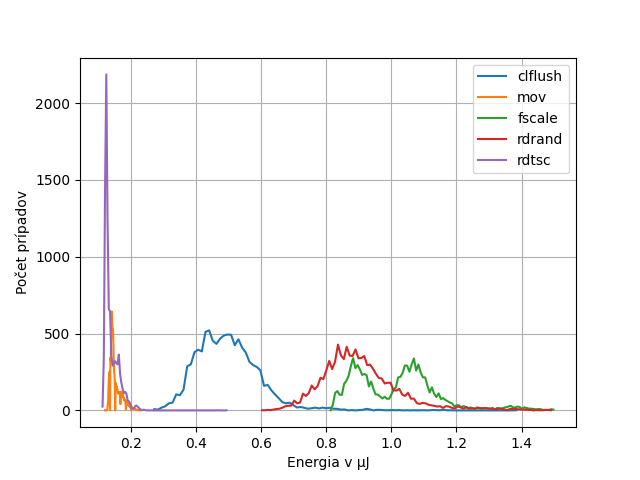
\includegraphics[scale=0.7]{./obrazky-figures/instr_comparison.png}
  \caption{Porovnanie spotreby vybraných inštrukcií.}
\end{figure}

Na obrázku \ref{img:instruction_comparison} je zobrazená energetická spotreba vybraných inštrukcií. V porovnaní s \cite{Platypus} je možné vidieť nielen odlišné
zoradenie inštrukcií podľa spotreby, ale aj rôzne prekrytie spotrieb. Inštrukcia \code{clflush} je najjednoduchšie rozlíšiteľná od ostatných, pričom \code{rdtsc} sa
od \code{mov} líši minimálne. Tabuľka \ref{tab:avg_energy_per_instruction} zobrazuje priemernú zmeranú spotrebu pre deväť rôznych inštrukcií.

\begin{table}\label{tab:avg_energy_per_instruction}
  \centering
  \caption{Priemerná zmeraná spotreba jednotlivých inštrukcií.}
  \begin{tabular}{ | l  r | }
    \hline
    Inštrukcia & Priemerná spotreba \\
    \hline
    \code{nop} & $0.08901 \mu J$ \\
    \code{inc} & $0.09315 \mu J$ \\
    \code{xor} & $0.09298 \mu J$ \\
    \code{mov} & $0.18403 \mu J$ \\
    \code{imul} & $0.17493 \mu J$ \\
    \code{fscale} & $1.10859 \mu J$ \\
    \code{rdrand} & $1.03944 \mu J$ \\
    \code{rdtsc} & $0.16500 \mu J$ \\
    \code{clflush} & $0.46188 \mu J$ \\
    \hline
  \end{tabular}
\end{table}

\subsection{Analýza spotreby energie pre rôzne operandy}
Podobne ako pri meraní spotreby inštrukcií, aj tu sa inštrukcie spúšťali $50000$-krát, avšak samotných stôp sa získavalo až $70000$.
Merala sa inštrukcia \code{imul}, pre ktorú sa podobne ako v \cite{Platypus} nastavil jeden operand na konštantu $8$, pričom druhý
sa nastavil na tri rôzne Hammingove váhy, konkrétne na $0$, $32$ a $64$. Bity operandov boli nastavené zoskupene, a teda jeden sled núl nasledovaný jedným sledom
jednotiek. Na obrázku \ref{img:imul_operands} je vidieť, že veľkosť operandov nemá žiaden výrazný dopad na rozloženie spotreby energie čítanej pomocou RAPL.

\begin{figure}\label{img:imul_operands}
  \centering
  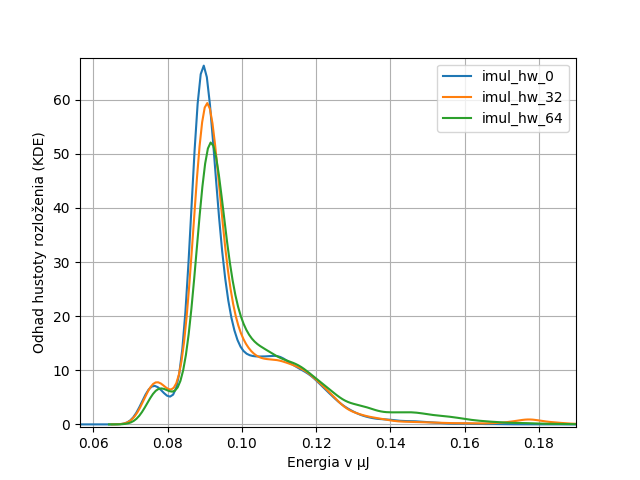
\includegraphics[scale=0.7]{./obrazky-figures/imul_operand_consumption.png}
  \caption{Porovnanie spotreby inštrukcie \code{imul} s operandami rôznej Hammingovej váhy.}
\end{figure}

\subsection{Skrytý kanál}
Jednou z vecí, ktoré monitorovanie spotreby procesora umožňuje, je vytvorenie skrytých kanálov za pomoci manipulácie spotreby. Na obrázku \ref{img:covert_channel}
je možné vidieť vizualizáciu správy zaslanej cez skrytý kanál medzi dvoma procesorovými vláknami. Zasielaná správa bol sled bitov \code{101001100}.
Vlákna neboli žiadnym spôsobom explicitne synchronizované, kvôli čomu je možné vidieť kľudový stav spotreby pred prvým preneseným bitom, ked prijímač iba naslúchal.

Počas implementácie skrytého kanálu sa prejavilo možné obmedzenie knižnice powercap, a to také, že nie je schopné získať informácie o spotrebe energie v prípade,
že je volaná v rámci dynamicky vytvoreného vlákna. Kvôli tomuto obmedzeniu sa pre účely merania spotrebovanej energie pristupovalo priamo k MSR cez
rozhranie \code{/dev/cpu/*/msr}.

\begin{figure}\label{img:covert_channel}
  \centering
  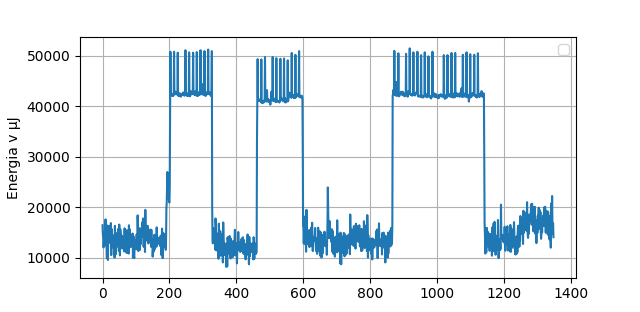
\includegraphics[scale=0.7]{./obrazky-figures/covert_channel.png}
  \caption{Vykreslenie sledu bitov \code{101001100} poslaných cez skrytý kanál za pomoci manipulácie spotreby procesora.}
\end{figure}

\section{Vyhodnotenie a záver}
V tejto práci som sa pokúsil o reprodukovanie vybraných častí práce \cite{Platypus}. \textbf{Experiment na rozlíšenie rôznych inštrukcií} na základe ich spotreby bol
čiastočne úspešný. Mnohé inštrukcie bolo možné rozlíšiť touto metódou, avšak pri inštrukciách s dostatočne podobnou spotrebou, ako sú napríklad trojica \code{imul},
\code{add} a \code{mov}, prípadne dvojica \code{nop} a \code{inc}, som nebol schopný s istotou rozlíšiť tieto inštrukcie.
\textbf{Experiment detekcie Hammingovej váhy operandov inštrukcií} bol neúspešný. Žiadny významný rozdiel v spotrebe medzi rôznymi Hammingovými váhami som nebol schopný
detegovať. Možným dôvodom je, že systém, na ktorom bol experiment vykonávaný neobsahuje čidlá pre meranie energie, ale spotrebu iba odhaduje.
V \cite{Platypus} sa uvádza, že architektúry Sandy bridge a Ivy bridge tieto čidlá neobsahujú, pričom môj testovací systém je postavený
na architektúre Haswell, čo je priamym nástupcom Ivy bridge. V danej publikácii architektúru Haswell netestovali a v iných publikáciách som
zmienku o najskoršom pridaní čidiel nenašiel. \textbf{Experiment skrytého kanálu} bol úspešný.


  \fi
  
  % Kompilace po částech (viz výše, nutno odkomentovat)
  % Compilation piecewise (see above, it is necessary to uncomment it)
  %\subfile{projekt-01-uvod-introduction}
  % ...
  %\subfile{chapters/projekt-05-conclusion}


  % Pouzita literatura / Bibliography
  % ----------------------------------------------
\ifslovak
  \makeatletter
  \def\@openbib@code{\addcontentsline{toc}{chapter}{Literatúra}}
  \makeatother
  \bibliographystyle{bib-styles/Pysny/skplain}
\else
  \ifczech
    \makeatletter
    \def\@openbib@code{\addcontentsline{toc}{chapter}{Literatura}}
    \makeatother
    \bibliographystyle{bib-styles/Pysny/czplain}
  \else 
    \makeatletter
    \def\@openbib@code{\addcontentsline{toc}{chapter}{Bibliography}}
    \makeatother
    \bibliographystyle{bib-styles/Pysny/enplain}
  %  \bibliographystyle{alpha}
  \fi
\fi
  \begin{flushleft}
  \bibliography{projekt-20-literatura-bibliography}
  \end{flushleft}

  % vynechani stranky v oboustrannem rezimu
  % Skip the page in the two-sided mode
  \iftwoside
    \cleardoublepage
  \fi

  % Prilohy / Appendices
  % ---------------------------------------------
  \appendix
\ifczech
  \renewcommand{\appendixpagename}{Přílohy}
  \renewcommand{\appendixtocname}{Přílohy}
  \renewcommand{\appendixname}{Příloha}
\fi
\ifslovak
  \renewcommand{\appendixpagename}{Prílohy}
  \renewcommand{\appendixtocname}{Prílohy}
  \renewcommand{\appendixname}{Príloha}
\fi
%  \appendixpage

% vynechani stranky v oboustrannem rezimu
% Skip the page in the two-sided mode
%\iftwoside
%  \cleardoublepage
%\fi
  
\ifslovak
%  \section*{Zoznam príloh}
%  \addcontentsline{toc}{section}{Zoznam príloh}
\else
  \ifczech
%    \section*{Seznam příloh}
%    \addcontentsline{toc}{section}{Seznam příloh}
  \else
%    \section*{List of Appendices}
%    \addcontentsline{toc}{section}{List of Appendices}
  \fi
\fi
  \startcontents[chapters]
  \setlength{\parskip}{0pt} 
  % seznam příloh / list of appendices
  % \printcontents[chapters]{l}{0}{\setcounter{tocdepth}{2}}
  
  \ifODSAZ
    \setlength{\parskip}{0.5\bigskipamount}
  \else
    \setlength{\parskip}{0pt}
  \fi
  
  % vynechani stranky v oboustrannem rezimu
  \iftwoside
    \cleardoublepage
  \fi
  
  % Přílohy / Appendices
  \ifenglish
    \input{projekt-30-prilohy-appendices-en}
  \else
    \input{projekt-30-prilohy-appendices}
  \fi
  
  % Kompilace po částech (viz výše, nutno odkomentovat)
  % Compilation piecewise (see above, it is necessary to uncomment it)
  %\subfile{projekt-30-prilohy-appendices}
  
\end{document}
